\section{Results and Discussion}
System-level simulation was performed with representative AI inference workloads.

\subsection{Standby Power}
Migrating cold data and checkpoints to the FeRAM-backed tier yields more than 30\% reduction in standby power.
This reduction arises from suppressing periodic DRAM refresh for inactive regions.

\subsection{Resume Latency}
FeRAM allows direct restore of checkpoints without full DRAM wake-up.
Resume latency is reduced to the $\mu$s range, enabling near-instant resume after power gating and improving energy efficiency for mobile edge AI.

\subsection{Endurance}
FeRAM endurance of $10^{12}$~writes/year fits within FeRAM capability for checkpoint traffic.

% ===== Fig.2: Access time vs. retention =====
\begin{figure*}[!t]
\centering
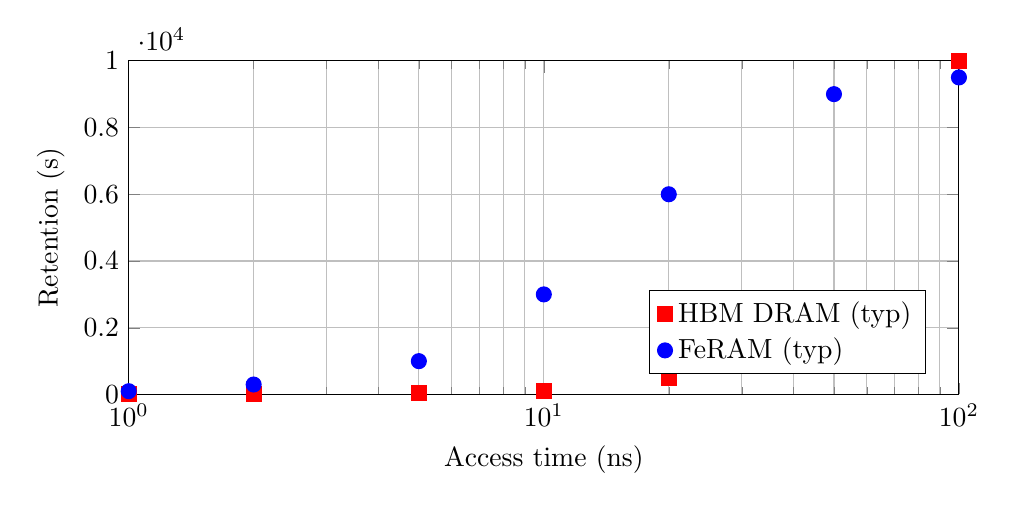
\begin{tikzpicture}
\begin{semilogxaxis}[
  width=\linewidth, height=0.48\linewidth,
  xmin=1e0, xmax=1e2, ymin=1e0, ymax=1e4,
  xlabel={Access time (ns)}, ylabel={Retention (s)},
  grid=both,
  legend style={at={(0.96,0.06)}, anchor=south east}, % 右下内側
  legend cell align={left}
]
% HBM = 赤四角(塗りつぶし)
\addplot+[only marks, mark=square*, mark size=2.7pt,
          mark options={fill=red, draw=red}]
coordinates {(1,10) (2,20) (5,50) (10,100) (20,500) (50,2000) (100,10000)};
\addlegendentry{HBM DRAM (typ)}

% FeRAM = 青丸(塗りつぶし)
\addplot+[only marks, mark=*, mark size=2.7pt,
          mark options={fill=blue, draw=blue}]
coordinates {(1,100) (2,300) (5,1000) (10,3000) (20,6000) (50,9000) (100,9500)};
\addlegendentry{FeRAM (typ)}
\end{semilogxaxis}
\end{tikzpicture}
\caption{Access time vs. retention. HBM: red filled squares; FeRAM: blue filled circles.}
\label{fig:retention_access}
\end{figure*}
